\section{时间序列的拓扑表示构建方法}

\subsection{引言与核心拓扑表示策略概述} % 修改后的引言
本章致力于探讨如何将时间序列数据转化为适用于拓扑数据分析(TDA)的表示形式,以便利用持久同调等工具提取其内在的拓扑特征。与传统的全局分析或简单统计不同,TDA能够捕捉数据的多尺度“形状”信息,对噪声具有鲁棒性,尤其适合处理复杂的非线性时间序列。然而,TDA的输入通常要求为点云或复形结构,这与原始的一维时间序列存在表示上的差异。

为应对这一挑战并深入挖掘时间序列的结构特性,本章将首先重点介绍两种具有代表性的拓扑表示构建策略:其一是\textbf{基于持续同调的时间序列倾斜处理方法(PHTSI)},通过对子序列施加时间相关的加权来增强时序依赖信息的捕获(详见3.2节);其二是\textbf{基于图的特征化时间序列构建方法},它允许灵活地融入领域知识来定制化持久同调的分析过程(详见3.3节)。

为了全面理解和实现这些方法,以及其他基于点云的TDA技术,本章后续将回顾将时间序列转化为高维点云的关键技术——\textbf{状态空间重构},特别是经典的时间延迟嵌入(TDE)及其参数选择问题,并简要介绍一些替代性的嵌入方案。
%
\subsection{基于持续同调的时间序列倾斜处理方法 (PHTSI)} % 原3.4节
在传统时间延迟嵌入及其直接变体之外,研究者亦致力于开发能够更全面捕捉时间序列特性,特别是高维拓扑信息与内在时序顺序信息的专门化方法。一个值得注意的进展来自严银凯等人(2024)\cite{JSJC202406009}提出的基于持续同调的倾斜时间序列分类(Persistent Homology Time Skew Incline, PHTSI)算法。该算法的核心创新在于其引入的“时间倾斜”(Time Skew)技术,旨在克服现有方法在提取时序顺序信息方面的不足,并增强对不同结构时间序列数据的适应性。
PHTSI算法的整体架构包含数据预处理、核心特征提取与分类三个主要阶段。其设计旨在从原始时间序列数据中发掘深层次的拓扑结构信息,并将其有效地应用于分类任务。接下来我们详细介绍这种算法。

\begin{figure}[thbp!]
    \centering
    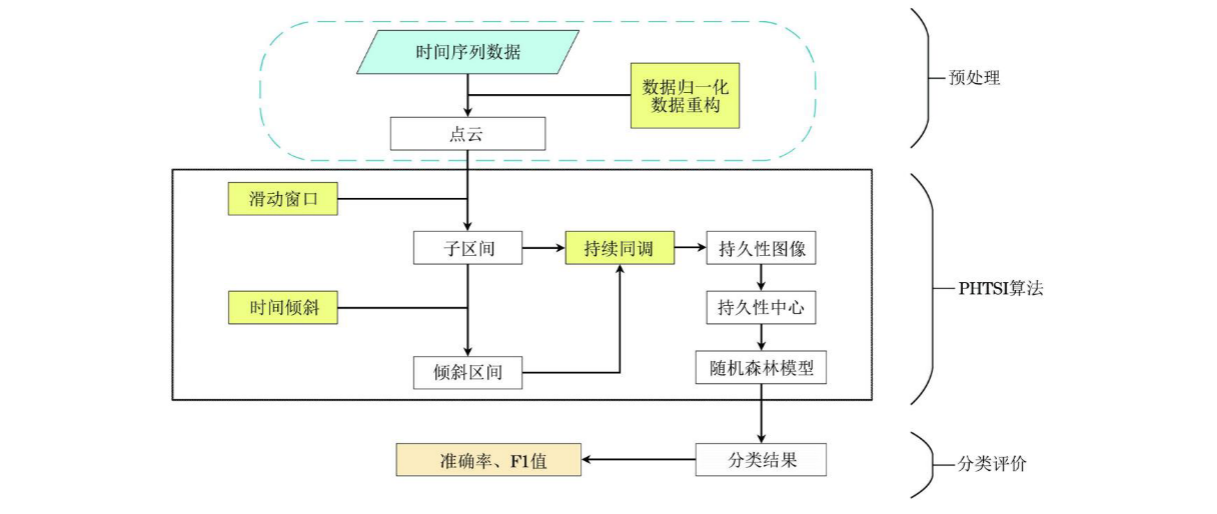
\includegraphics[width=1.0\textwidth]{figure/严银凯示意图.png}
    \caption{PHTSI算法示意图。}
    \label{fig:phtsi_algorithm}
\end{figure}

\paragraph*{步骤一:数据预处理}
在进行特征提取之前,原始时间序列数据需经过一系列预处理步骤,以确保数据的规范性并构建适用于拓扑分析的表示形式。首先需要做的是进行数据规范化,因为时间序列的数据通常的量纲不一致,通常会影响后续的分析过程,因此需要将数据尺度统一到特定区间。例如采用最小-最大规范化方法,将数据缩放到 $[0, 1]$ 的范围内。消除不同序列之间因为量纲差异可能导致的计算偏差问题。

随后需要将一维时间序列转化为二维的点云结构,在本章的开头就介绍了点云构造方法,对于原始时间序列中的每一个数据点 $a_t^i$,通过结合其后续点的差分信息,构造一个二维向量 $q_t^i = (a_t^i, a_{t+1}^i - a_t^i)$。这样的转换不仅保留了原始数据点的值,还融入了其局部变化趋势,初步揭示了序列的动态特性。
%
\paragraph*{步骤二:核心特征提取}
在构造完成点云之后,我们需要采用滑动窗口子序列划分方法,具体的做法是选择固定尺寸的滑动窗口及预设的滑动步长,将前一步构建的二维点云序列分割成若干个等长的子序列片段。这种局部化的处理方式有助于捕捉时间序列在不同阶段的局部模式,同时也能有效控制后续持久同调计算的复杂度。设窗口大小为 $w$ ,滑动步长为 $d_{step}$ (此处用 $d_{step}$ 以区别嵌入维度 $d$),则第 $i$ 个原始序列的第 $j$ 个子序列 $W_i^{j, 1}$ 可以表示为:
\begin{equation}
    W_i^{j, 1}=\left(q_{d_{step} \cdot j-d_{step}+1}^i, q_{d_{step} \cdot j-d_{step}+2}^i, \ldots, q_{d_{step} \cdot j-d_{step}+w}^i\right)
\end{equation}

接下来就是非常重要的时间序列倾斜方法,其目的是对子序列进行结构增强,用来揭示更丰富的时序依赖信息。“时间倾斜”是本研究中创新采用的一种策略,旨在通过对时间序列子区间内的点云施加与时间位置相关的加权,从而生成具有不同结构特性的新序列。
假设我们有一个从原始时间序列中提取的子区间(或称为滑动窗口内的点云),记为 $S$ 。该子区间由 $W$ 个按时间顺序排列的点组成:
\begin{equation}
    S=\left(p_1, p_2, \ldots, p_W\right)
\end{equation}
其中,$p_l$ 代表子区间内第 $l$ 个时间点对应的数据点(可能是一个向量,例如 $p_l=x\left(t_l\right)$ )。
时间倾斜方法通过将此子区间 $S$ 与两个不同的时间依赖函数 $f_1$ 和 $f_2$ 进行逐点乘法(或加权)来实现。

第一个倾斜变换采用线性函数 $f_1(k)=k$(其中 $k$ 为点在子序列中的序号,从1到 $w$ ),作用于子序列中的每个点 $q_k^{\prime}$(代表 $W_i^{j, 1}$ 中的第 $k$ 个点):
$$
    W_i^{j, 2}=\left(1 \cdot q_1^{\prime}, 2 \cdot q_2^{\prime}, \ldots, w \cdot q_w^{\prime}\right)
$$
此变换增强了子序列中后续点的影响。
第二个倾斜变换采用线性函数 $f_2(k)=w-k+1$ ,作用于子序列中的每个点 $q_k^{\prime}$ :
$$
    W_i^{j, 3}=\left(w \cdot q_1^{\prime},(w-1) \cdot q_2^{\prime}, \ldots, 1 \cdot q_w^{\prime}\right)
$$
此变换则增强了子序列中初始点的影响。
通过这种方式,原始子序列 $W_i^{j, 1}$ 及其两个倾斜版本 $W_i^{j, 2}$ 和 $W_i^{j, 3}$ 共同构成了后续拓扑分析的基础,使得算法能够从多个角度审视数据的内在结构。
到这里为止都是为了第四章的持续同调计算和持久性图生成做准备,后续具体内容会在第四章详细讲解。

\subsection{基于图的特征化时间序列表示} % 原3.5节
在标准的时间序列拓扑表示构建方法之外,为了更灵活地融入领域特定知识并优化持久同调的分析效果,Heo 与 Jung \cite{2} 近期提出了一种新颖的框架。该方法的核心在于引入了“特征化时间序列 (featured time series)”与“影响向量 (influence vector)”的概念,旨在通过调整时间序列的图表示来定制化持久同调的计算过程。

首先,一个特征化时间序列 $(\hat{T}, g)$ 由两部分构成:其一是特征增强的时间序列 $\hat{T}$,它将原始时间序列 $T$ 与一个特征组件 $T_f$ 配对,即 $\hat{T}(t) = (T(t), T_f(t))$。这里的特征组件 $T_f(t)$ 可以包含与单个时间点 $T(t)$ 相关的0阶特征(例如,某时刻的湿度状况)以及与相邻时间点对 $\{T(t_k), T(t_{k+1})\}$ 相关的1阶特征(例如,温度变化的幅度)。这些特征通常来源于特定领域的知识。其二是影响向量 $g$,它是一个非负实值函数,为每一个定义的特征(以及无特征状态)赋予一个“影响值”,用以量化该特征在后续分析中的重要性 。我们先引入一个存在异常区域的时间序列:
\begin{figure}[thbp!]
    \centering
    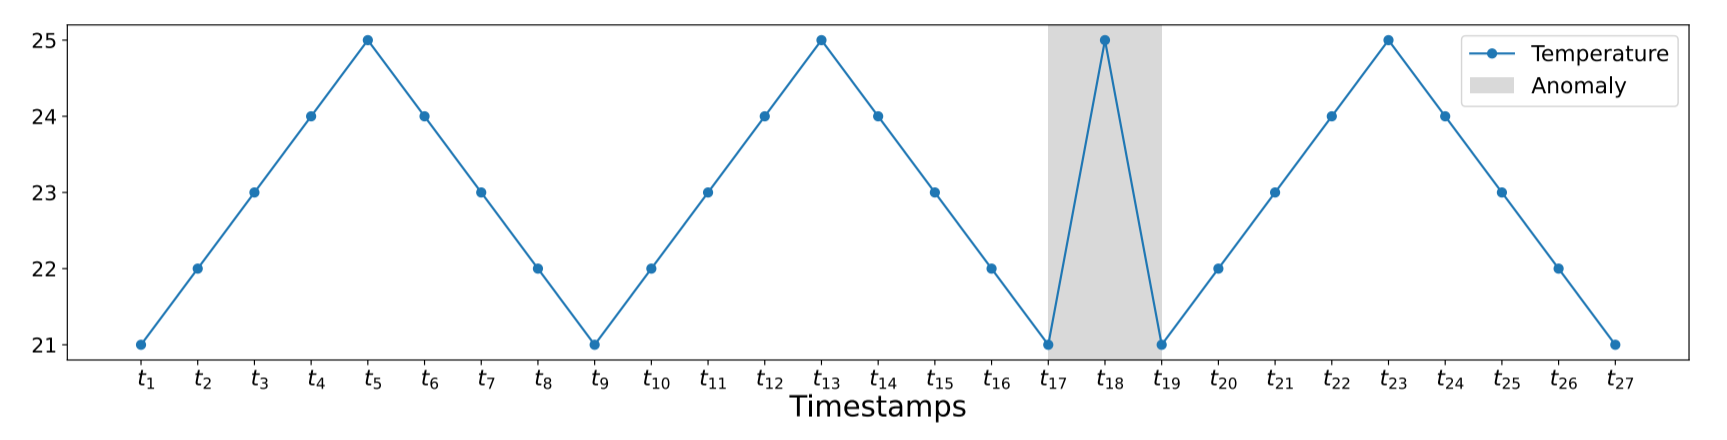
\includegraphics[width=1.0\textwidth]{figure/时间序列例子.png}
    \caption{存在异常的温度时间序列}
    \label{fig:phtsi_algorithm}
\end{figure}

该方法接着利用特征化时间序列 $(\hat{T}, g)$ 来构建一个加权图 $G=(V,E,\hat{W}_V,\hat{W}_E)$。其中,顶点集 $V$ 由时间序列中的观测值构成,边集 $E$ 通常连接连续的观测值。关键在于顶点权重函数 $\hat{W}_V$ 和边权重函数 $\hat{W}_E$ 的计算。它们并非简单地基于原始序列的频率,而是通过结合特征的出现次数和影响向量 $g$ 来确定。具体地,设 $F^0 = \{r_1, ..., r_m\}$ 为0阶特征集,$F^1 = \{s_1, ..., s_l\}$ 为1阶特征集。定义0阶计数矩阵 $C_0=(c_{ij}^0)$,其中 $c_{ij}^0$ 表示顶点 $v_i$ 与特征 $r_j$ (或无0阶特征状态 $\emptyset^0$) 在 $\hat{T}$ 中共同出现的次数。类似地,定义1阶计数矩阵 $C_1=(c_{ij}^1)$,其中 $c_{ij}^1$ 表示边 $e_i$ 与特征 $s_j$ (或无1阶特征状态 $\emptyset^1$) 在 $\hat{T}$ 中共同出现的次数。若影响向量 $g$ 对应0阶和1阶特征的分量分别为 $\vec{g_0} = (g(\emptyset^0), g(r_1), ..., g(r_m))$ 和 $\vec{g_1} = (g(\emptyset^1), g(s_1), ..., g(s_l))$,则顶点 $v_i$ 的权重和边 $e_i$ 的权重(也称为加权频率 $\hat{f}_{e_i}$)可以计算为:
\begin{equation}
    \hat{W}_V(v_i) = (C_0 \cdot \vec{g_0})_i
\end{equation}
\begin{equation}
    \hat{W}_E(e_i) = \hat{f}_{e_i} = (C_1 \cdot (\vec{g_1} + \vec{1}))_i
\end{equation}
其中 $\vec{1}$ 是全1向量,用于确保在 $\vec{g_1}=\vec{0}$ 时边权重与传统频率定义一致 。下面给出加权图的一个示例:
\begin{figure}[thbp!]
    \centering
    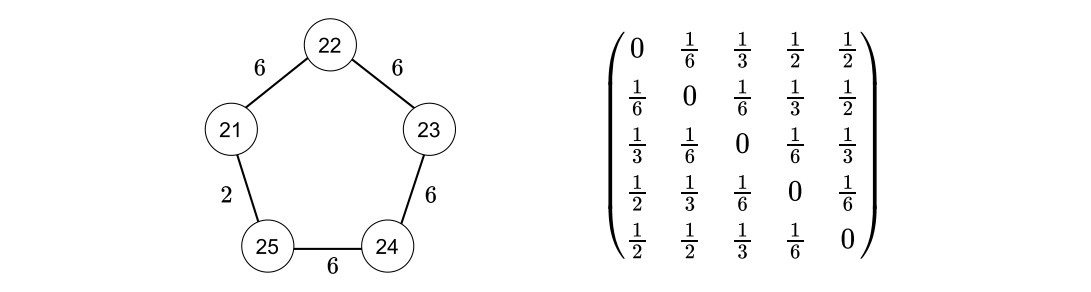
\includegraphics[width=1.0\textwidth]{figure/第三章加权图示意.png}
    \caption{时间序列的加权图与距离矩阵}
    \label{fig:phtsi_algorithm}
\end{figure}

随后,基于这个加权的图 $\hat{G}^g$,定义了节点间的距离度量 $\hat{d}$。对于图中的一条边 $e=\{a,b\}$,其长度 $L^g(e)$ 不仅考虑了其加权频率的倒数 $(\hat{W}_E(e))^{-1}$,还通过一个激活函数 $\rho$ (如 $\rho(z)=1-e^{-z^2}$ 对于 $z \ge 0$) 引入了与该边连接的两个顶点 $a,b$ 的加权频率 $\hat{W}_V(a)$ 和 $\hat{W}_V(b)$ 的影响:
\begin{equation}
    L^g(e) = (\hat{W}_E(e))^{-1} - \alpha (\rho(\hat{W}_V(a) + \hat{W}_V(b)))
\end{equation}
其中 $\alpha = \min_{e' \in E} (\hat{W}_E(e'))^{-1}$ 是一个归一化因子,确保边长非负。两个顶点 $v,w$ 之间的距离 $\hat{d}(v,w)$ 则定义为连接它们的最短路径上所有边长度 $L^g(e)$ 之和 。
\begin{equation}
    \hat{d}(v,w) = \min_{p: v \leadsto w} \left\{ \sum_{e \in p} L^g(e) \right\}
\end{equation}
这个经过特征和影响向量调整的距离度量 $(V, \hat{d})$ 构成了计算持久同调(例如通过Vietoris-Rips滤过)的基础。通过改变影响向量 $g$,研究者可以探索不同领域知识对时间序列拓扑结构的影响,具体构造方式如下图。Heo 与 Jung 最后证明了这种方法的一个重要性质:持久性图对于影响向量 $g$ 的变化是稳定的,即满足 $D_B(\text{dgm}_p(g), \text{dgm}_p(g')) \le C ||g-g'||_\infty$,其中 $D_B$ 是瓶颈距离,$C$ 是一个常数。这种稳定性保证了该增强方法在调整领域知识影响时的鲁棒性和结果的可靠性。
\clearpage
\begin{figure}[thbp!]
    \centering
    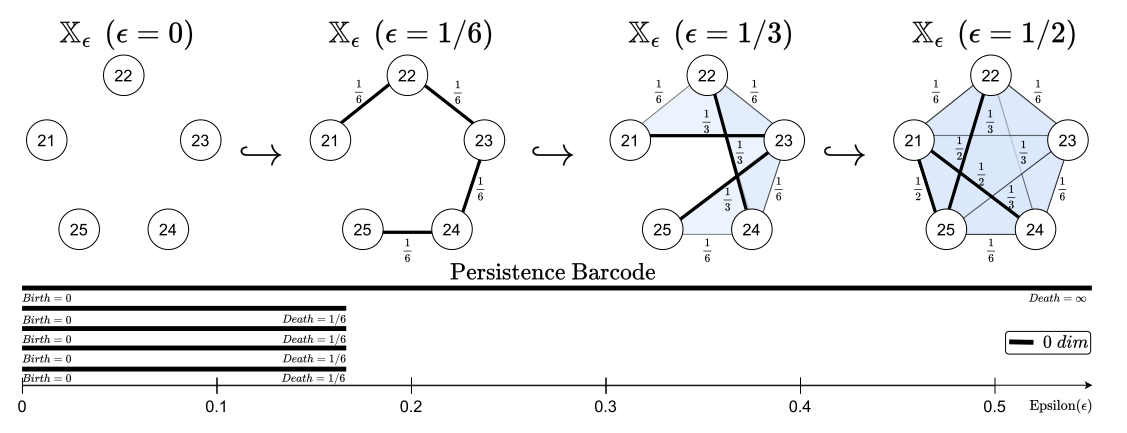
\includegraphics[width=0.8\textwidth]{figure/特征化时间序列.png}
    \caption{Rips过滤和条码图}
    \label{fig:phtsi_algorithm}
\end{figure}


之后我们通过一个表格来对比传统的点云嵌入方法与Heo \& Jung的特征化时间序列方法。表格中列出了两者在核心目标、距离度量来源、领域知识整合、调整机制、增强体现和理论稳定性等方面的主要区别。
\begin{table}[htbp]
    \centering
    \caption{传统点云嵌入与Heo \& Jung特征化时间序列方法的简明对比}
    \label{tab:embedding_comparison_concise_new}
    \begin{tabular}{>{\raggedright\arraybackslash}p{0.25\textwidth} >{\raggedright\arraybackslash}p{0.35\textwidth} >{\raggedright\arraybackslash}p{0.35\textwidth}}
        \toprule
        \textbf{比较维度}                          & \textbf{传统点云嵌入 (以TDE为例)} & \textbf{Heo \& Jung 的特征化方法} \\
        \midrule
        核心目标/输出                                &
        在欧几里得空间($\mathbb{R}^m$)中重构几何点云,代表系统状态。 &
        构建一个赋权图,并基于此定义一个可调整的度量空间 $(V, \hat{d})$ 作为拓扑分析输入。                                               \\
        \addlinespace
        距离度量来源                                 &
        通常是嵌入点之间的欧几里得距离。                       &
        基于图的边/点权重(由特征和影响向量决定)定义的最短路径距离 $\hat{d}(v,w)$。                                                  \\
        \addlinespace
        领域知识整合                                 &
        通常不直接在构造中融入,主要通过参数选择间接体现。              &
        通过“特征化时间序列”和“影响向量”显式、量化地融入距离度量的计算中。                                                             \\
        \addlinespace
        调整机制                                   &
        主要调整嵌入维度 $d$ 和时间延迟 $\tau$。             &
        主要调整“影响向量” $g$,改变特征对距离度量的影响。                                                                    \\
        \addlinespace
        “增强”体现                                 &
        优化参数以期更好地“展开”吸引子。                      &
        通过影响向量主动“调制”点间距离,使度量空间更能反映关注的结构。                                                                \\

        \bottomrule
    \end{tabular}
\end{table}

\subsection{时间序列的点云转换基础} % 新的小节,整合原3.2和3.3
上述特定方法以及其他多种基于点云的拓扑数据分析技术,其前提都是将原始的一维时间序列有效地转化为高维空间中的点云表示。状态空间重构为实现这一目标提供了核心的理论框架,其中时间延迟嵌入(TDE)是最为经典和基础的技术。本节将回顾这些基础方法及其相关的参数选择问题。

\subsubsection{状态空间重构概览} % 来自原3.2节的引言部分
我们需要将观测到的时间序列数据重构系统动力学状态空间,并构建其拓扑表示的方法.在许多科学和工程领域,我们面对的是复杂的动态系统,但往往只能观测到系统的一个或少数几个变量随着时间而变化,这种观测导致我们难以理解分析系统完整行为,所以我们需要从有限的,可能带有噪声的观测数据中,推断出驱动系统演化的潜在高维信息.传统的线性时间序列分析方法虽然在某些情况下有效,但往往难以捕捉复杂系统所固有的非线性特征和相互作用.状态空间重构是一个非常的好的解决办法,其基本思想是将低维的时间序列数据,通过特定的嵌入技术,转化为一个高维空间中的几何对象,这个重构出的状态空间在理想情况下能保持原始系统动力学的主要拓扑和几何特性.在众多状态空间重构技术中,时间延迟嵌入(TDE)扮演着基石性的角色.

\subsubsection{时间延迟嵌入 (TDE) 及其理论基础}
\paragraph{Takens 嵌入定理} % 原3.2.1节
TAKENS嵌入定理(Takens' Embedding Theorem)\cite{takens2006detecting}是由荷兰数学家Floris Takens在1981年提出的一个重要数学定理,主要应用于动力系统和时间序列分析领域。它提供了一种从单一标量时间序列数据中重构原始动力系统相空间的方法,尤其在研究混沌系统和非线性动力学时具有深远意义。

在介绍定理之前我们先来介绍两个基本概念:
\begin{itemize}
    \item \textbf{相空间(Phase Space)}: 动力系统的状态空间,描述系统所有可能状态的集合。对于一个n维动力系统,相空间是n维的。
    \item \textbf{吸引子(Attractor)}: 动力系统在长时间演化后趋向的状态或轨迹集合。吸引子可以是点、周期轨道或更复杂的结构,如奇异吸引子。
\end{itemize}
TAKENS嵌入定理的核心思想是,通过对时间序列进行适当的嵌入,可以在高维空间中重构出原始动力系统的相空间结构。具体来说,假设我们有一个一维时间序列$x(t)$,它是一个动力系统在时间上的投影。TAKENS定理指出,如果我们选择合适的\textbf{嵌入维度 $d$} 和\textbf{时间延迟 $\tau$},那么通过以下方式构造的 $d$ 维向量序列可以近似重构原始动力系统的相空间:
\begin{equation}
    \mathbf{x}_i = (x(t_i), x(t_{i+\tau}), x(t_{i+2\tau}), \ldots, x(t_{i+(d-1)\tau}))
\end{equation}
其中,$i$是时间序列的索引,$t_i$是时间点。

TAKENS定理的直观解释是:由于确定性动力系统中各个状态变量是相互耦合的,当前观测值及其过去(或未来)的延迟值序列中,蕴含了关于当前未被直接观测到的其他状态变量的信息.
补充: Sauer等人进一步完善了嵌入维度的条件,指出嵌入维度 $d$ 需要满足 $d \geq 2D_{sys}+1$, 其中 $D_{sys}$ 是原始动力系统吸引子的维数。这个定理的一个重要结论是,只要嵌入维度足够大,就可以通过重构的相空间来恢复原始系统的动力学行为,包括吸引子结构和混沌特性.

\paragraph{时间延迟嵌入 (TDE) 原理与实现} % 原3.2.2节
时间延迟嵌入(Time Delay Embedding, TDE) 是一种将一维时间序列数据转化为高维点云的技术,基于 Takens 嵌入定理。TDE 的基本思想是通过引入时间延迟和嵌入维度,将时间序列中的每个观测值与其过去的观测值组合成一个高维向量,从而重构出系统的相空间。这种方法能够捕捉到系统的非线性动力学特征,如周期性、混沌行为等。
TDE 的基本原理是将一维时间序列 \( s(t) \) 通过引入时间延迟 \( \tau \) 和嵌入维度 \( d \),转化为高维向量:
\begin{equation}
    \vec{x}(t) = \left[ s(t), s(t - \tau), s(t - 2\tau), \dots, s(t - (d - 1)\tau) \right]
\end{equation}
这些向量构成的集合形成了一个高维点云,即重构的相空间。根据Takens定理(及其后续改进),当嵌入维度 $d$ 足够大(例如 $d \geq 2D_{sys} + 1$,其中 $D_{sys}$ 为原始系统吸引子的维数)时,重构的相空间与原始系统的相空间在拓扑上是等价的。这种重构使得我们可以从单一观测变量中恢复系统的非线性动力学行为,例如吸引子结构或混沌特性。点云中的每个点代表系统在某时刻的状态,而点云的几何形状则反映了系统的长期演化规律。
%插入图片
\begin{figure}[thbp!]
    \centering
    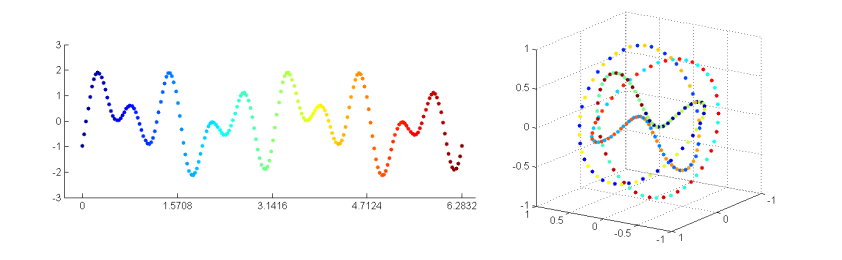
\includegraphics[width=1.0\textwidth]{figure/滑动窗口嵌入示意图、.png}
    \caption{周期性数据滑动窗口嵌入点云示意图}
    \label{fig:tde_example}
\end{figure}

\subsubsection{TDE 关键参数选择}
\paragraph{嵌入维度参数 $d$ 的选择} % 原3.2.3节
时间延迟嵌入(TDE)中嵌入维度 $d$ 的选择,直接决定了重构状态向量 $\vec{y}(t) = [x(t), \dots, x(t+(d-1)\tau)]$,对能否有效重构系统动力学至关重要。一个充分的 $d$ 值是保证重构空间能真实反映原始吸引子拓扑结构的基础。

若 $d$ 值选取 \textbf{过低},重构空间不足以完全“展开”高维吸引子,会导致原本分离的轨迹因投影而错误地靠近,产生所谓的 “伪近邻” (FNN)。这种拓扑结构的扭曲会严重影响后续基于重构空间的分析。

反之,若 $d$ 值选取 \textbf{过高},则会引入 “维度灾难” 问题。在有限数据下,高维空间的数据点变得稀疏,降低了依赖局部密度估计的分析方法(如关联维计算)的可靠性。同时,高维度也增加了计算负担并可能放大噪声。

因此,目标是找到最小的充分嵌入维度 $d_{min}$,它既能完全展开吸引子(消除FNN),又能避免不必要的高维问题。虽然Takens等理论给出了维度的理论下界(如 $d \ge 2D_{sys}+1$ 或 $d > 2D_A$, 其中 $D_A$ 为吸引子的某种维度度量),但通常需要根据数据进行估计。

实践中常用数据驱动方法估计 $d$。伪近邻法 (FNN)\cite{rhodes1997false}通过考察随着维度从当前值增加到 $d+1$(原文笔误,应为从一个维度 $d'$ 增加到 $d'+1$),近邻点对的距离是否显著增大来判断维度是否充分。当伪近邻比例降至阈值以下时,对应的 $d$ 可视为一个充分估计。Cao方法\cite{cao1997practical} 是对FNN的改进,通过分析统计量 $E1(d)$(邻近点距离的平均相对变化率)随 $d$ 的饱和行为来确定 $d$,并用 $E2(d)$ 辅助判断数据是否具有确定性。

总之,$d$ 的选择是一个需要在保证拓扑嵌入有效性与避免高维问题之间进行权衡的经验过程。通常需要结合使用多种估计方法,并考虑数据特性(长度、噪声)及分析目标。对估计值附近的 $d$ 进行敏感性分析,检验后续结果的稳定性,是验证选择合理性的常用手段。以下是一些常用的方法:

% --- End of LaTeX Snippet ---

\begin{table}[h!] % 使用 [h!] 尝试将表格放置在此处
    \centering % 表格居中
    \caption{时间延迟嵌入嵌入维度($d$)选择方法对比}
    \label{tab:embedding_dimension_methods_no_pros_cons_new}
    \begin{tabular}{
        >{\raggedright\arraybackslash}m{3cm} % 方法名称 (左对齐,自动换行)
        >{\raggedright\arraybackslash}m{4.5cm} % 核心原理 (左对齐,自动换行)
        >{\raggedright\arraybackslash}m{5cm}  % 原理阐释 (左对齐,自动换行)
        >{\raggedright\arraybackslash}m{4cm}  % 常用判据 (左对齐,自动换行)
        }
        \toprule % 顶部线条
        \textbf{方法名称}                        & \textbf{核心原理}             & \textbf{原理阐释}                                          & \textbf{常用判据/解释}                                                                       \\
        \midrule % 中间线条

        伪近邻法 (FNN) \cite{rhodes1997false}    & 邻近点在维度增加时的相对距离变化          & 维度不足时,投影导致假邻居;维度足够时,假邻居会散开,真邻居保持靠近                     & FNN随 $d$ 增加首次降至零或小阈值                                                                   \\
        \addlinespace % 增加行间距

        Cao方法\cite{cao1997practical}         & 近邻点对距离相对变化率的平均值 ($E1(d)$) & 旨在改进FNN,减少对阈值的依赖;观察变化率何时稳定                             & 绘制 $E1(d)$ 曲线,寻找其趋于平稳的 $d$ 值 。$E2(d)$ 用于区分确定性与随机性                                      \\
        \addlinespace

        符号动力学/熵方法\cite{matilla2021selection} & 符号序列的熵                    & 利用熵度量信息量或依赖性随参数的变化;将嵌入参数 $d, \tau$ 与最优时间窗口 $\tau_w$ 关联 & 寻找使熵最大化($\tau^*$)和最小化($\tau_w$)的延迟,通过 $\tau_w=(d-1)\tau^*$ (或类似形式)确定 $d$               \\
        \addlinespace

        Takens/Sauer 定理 (理论基础)               & 保证嵌入的微分同胚性                & 足够高的维度能“展开”吸引子,保持拓扑结构                                  & 理论要求 $d > 2D_{sys}$ (Takens改进后) 或 $d > 2D_A$ (Sauer),其中 $D_{sys}$ 为系统维数,$D_A$ 为吸引子某种维数 \\

        \bottomrule % 底部线条
    \end{tabular}
    \par % 确保表格后的文本在新行开始
    \vspace{0.5cm} % 在表格后增加一些垂直空间
\end{table}

下面我来介绍一下cao方法在论文中的运用:
曹亮月\cite{cao1997practical}提出的确定标量时间序列最小嵌入维数 $d_{min}$ 的方法,其核心思想是避免传统方法中主观参数的选择。该方法首先定义一个量 $a(i,d)$:
\begin{equation}
    a(i,d) = \frac{||y_i(d+1) - y_{n(i,d)}(d+1)||}{||y_i(d) - y_{n(i,d)}(d)||}
\end{equation}
其中 $y_i(d)$ 是 $d$ 维重构相空间中的点,$y_{n(i,d)}(d)$ 是其最近邻。然后计算 $a(i,d)$ 的均值 $E(d)$:
\begin{equation}
    E(d) = \frac{1}{N-d\tau}\sum_{i=1}^{N-d\tau} a(i,d)
\end{equation}
并考察其变化率 $E1(d)$:
\begin{equation}
    E1(d) = E(d+1)/E(d)
\end{equation}
当 $d$ 大于某个值 $d_0$ 后,$E1(d)$ 趋于饱和,此时 $d_0+1$ 即为最小嵌入维数。为区分确定性与随机信号,还引入了 $E^*(d)$:
\begin{equation}
    E^*(d) = \frac{1}{N-d\tau}\sum_{i=1}^{N-d\tau} |x_{i+d\tau} - x_{n(i,d)+d\tau}|
\end{equation}
及其变化率 $E2(d)$:
\begin{equation}
    E2(d) = E^*(d+1)/E^*(d)
\end{equation}
对于随机数据,$E2(d)$ 对所有 $d$ 均约等于1。下表总结了论文中部分实验结果:

\begin{table}[h!]
    \centering
    \caption{曹氏方法实验结果选例}
    \label{tab:cao_results_adjusted} % 建议修改label以区分
    % 请确保在导言区有 \usepackage{array}
    \begin{tabular}{|l|l|l|>{\raggedright\arraybackslash}p{3.5cm}|} % 修改了第四列的定义
        \hline
        \textbf{系统}                 & \textbf{采样点个数} & \textbf{Cao方法 $d_{min}$} & \textbf{备注/FNN对比}        \\
        \hline
        Hénon 吸引子                   & 1000 \& 10000  & 2                        & 结果对数据长度不敏感               \\
        \hline
        Ikeda 吸引子                   & 1000 \& 10000  & 4                        & 1000点时FNN结果不稳定           \\
        \hline
        Lorenz 吸引子                  & 1000 \& 10000  & 3                        & 结果稳定                     \\
        \hline
        随机有色噪声                      & 1000 \& 10000  & N/A ($E2 \approx 1$)     & FNN方法会误判为低维混沌            \\
        \hline
        Mackey-Glass ($\Delta=100$) & 1000 \& 10000  & 17                       & FNN方法结果偏小 ($\sim$6)且依赖参数 \\
        \hline
        特定四维映射                      & 1000 \& 10000  & 4                        & 1000点时FNN无法区分            \\
        \hline
        实验激光数据                      & 1000           & 7                        & FNN结果在$d=7$后不稳定          \\
        \hline
    \end{tabular}
\end{table}

曹亮月通过对Hénon映射、Ikeda映射、Lorenz吸引子、随机有色噪声、高维Mackey-Glass方程、特定四维映射及真实激光数据等多种时间序列的实验验证了其方法的有效性。实验结果表明,该方法不仅能准确确定不同动力系统的最小嵌入维数 $d_{min}$,且对数据长度不敏感;尤为重要的是,它能有效区分确定性混沌与随机信号(如随机有色噪声,此时$E2(d) \approx 1$),并在处理高维系统(如Mackey-Glass)时显著优于传统的虚假最近邻(FNN)方法,后者在这些情况下常给出偏低或不稳定的结果且依赖于参数选择 。这些实验共同证明了曹氏方法在确定嵌入维数方面的鲁棒性、客观性和广泛适用性。

\paragraph{时间延迟参数 $\tau$ 的选择} % 原3.2.4节
在利用时间延迟嵌入技术重构复杂系统相空间的过程中,除了选择合适的嵌入维度 $d$ 之外,时间延迟参数 $\tau$ 的选取同样是\textbf{至关重要}的一环。它直接决定了构成嵌入向量 $\vec{y}(t) = [x(t), x(t-\tau), \dots, x(t-(d-1)\tau)]$ (此处统一符号,原文为 $x(t+\tau), \dots, x(t+(m-1)\tau)$)各分量之间的时间间隔。一个恰当的 $\tau$ 值是保证重构相空间能够有效“展开”原始动力系统吸引子,并保持其拓扑结构不变性的关键因素之一。

选择一个过小的 $\tau$ 值,会导致嵌入向量的相邻分量之间线性相关性过强,信息冗余度高。此时,$x(t)$ 与 $x(t-\tau)$ 非常接近,它们并未提供足够多的“新”信息来区分邻近的轨迹段。结果是,重构出的吸引子可能仍然是“折叠”或“挤压”在一起的,未能充分展现其在高维空间中的真实几何形态,这无疑会扭曲我们对系统动力学行为的理解。

相反,如果选择一个过大的 $\tau$ 值,虽然可以保证各分量之间的线性无关性甚至统计独立性,但 $x(t)$ 与 $x(t-(d-1)\tau)$ 之间可能已经失去了系统内在的动力学关联。这相当于在时间上跳跃得太远,使得嵌入向量无法捕捉到系统轨迹的连续演化特征和确定性结构,重构出的相空间可能变得杂乱无章,甚至接近随机噪声的表现,同样无法真实反映原始动力学。

因此,$\tau$ 的选择面临着一个\textbf{核心的权衡}:既要足够大以确保嵌入向量的各分量包含足够独立的信息,从而有效展开吸引子;又要足够小以保留系统随时间演化的内在关联性与动力学规律。一个不恰当的 $\tau$ 值将直接影响后续所有基于重构相空间的分析,包括分形维数的计算、Lyapunov 指数的估计、系统的预测精度以及噪声抑制的效果等。鉴于其对整个相空间重构质量和后续分析有效性的\textbf{决定性影响},如何合理地选择时间延迟 $\tau$ 成为了时间序列非线性分析中的一个基本且关键的问题。下面将展示几种常用的 $\tau$ 值选择策略及其背后的原理。

\begin{table}[h!]
    \centering
    \caption{时间延迟嵌入时间延迟 ($\tau$) 选择方法对比}
    \label{tab:time_delay_tau_methods_compare_new}
    \begin{tabular}{
        >{\raggedright\arraybackslash}m{3cm}
        >{\raggedright\arraybackslash}m{4.5cm}
        >{\raggedright\arraybackslash}m{5cm}
        >{\raggedright\arraybackslash}m{4cm}
        }
        \toprule
        \textbf{方法名称}                              & \textbf{核心原理} (分析的度量)                 & \textbf{原理阐释} (为何有效)                        & \textbf{常用判据/解释}                                                                \\
        \midrule

        自相关函数 (ACF)\cite{kantz2003nonlinear}       & 时间序列与其滞后版本间的线性相关性                     & 寻找 $x(t)$ 与 $x(t+\tau)$ 线性无关的最小延迟           & $\tau$ 取 ACF 首次降至零 或首次降至 $1/e \approx 0.37$ 的值                                  \\
        \addlinespace

        平均互信息 (AMI)\cite{wallot2018calculation}    & $x(t)$ 与 $x(t+\tau)$ 之间的统计依赖性 (信息论度量) & 寻找 $x(t)$ 与 $x(t+\tau)$ 共享信息量最少的延迟,以捕捉非线性结构 & $\tau$ 取 AMI 函数 $I(\tau)$ 的第一个局部最小值                                             \\
        \addlinespace

        C-C 方法 (基于关联积分)\cite{cai2008determination} & 分析关联积分在不同 $\tau, d$ 下随邻域半径 $r$ 的变化    & 通过检验不同时间窗内数据的统计独立性与几何展开程度寻找最优参数             & 寻找特定统计量(如 $\Delta \bar{S}_2(t)$ 或 $\sigma_{cor}(t)$)首次穿零或达极小值对应的 $t$ (即 $\tau$) \\
        \addlinespace

        几何/直观方法                                    & 观察时间序列图或相图的特征时间尺度                     & 基于对系统动力学行为的先验知识或直观观察估计                      & $\tau$ 常取为主要周期或特征时间的某个分数(如 1/4 到 1/10)                                          \\
        \bottomrule
    \end{tabular}
    \par
    \vspace{0.5cm}
    \textit{注意:选择 $\tau$ 与选择 $d$ 密切相关。实际应用中 $\tau$ 的选择常带有启发性,需测试不同值的影响。AMI 通常被认为是较优选择。}
\end{table}

\textbf{相关实验}: Wallot 和 Mønster(2018)\cite{wallot2018calculation} 该实验选择时间嵌入参数时,首先使用平均互信息(AMI)确定延迟参数 $\tau$。对于一维时间序列 $x(t)$,AMI 的计算公式为
$$I(x(t),x(t+\tau))=\sum_{i,j}p_{ij}(\tau)\log\left(\frac{p_{ij}(\tau)}{p_{i}p_{j}}\right)$$
其中 $p_i$ 是数据点在直方图第 $i$ 个bin的概率,$p_{ij}(\tau)$ 是 $x(t)$ 在 bin $i$ 且 $x(t+\tau)$ 在 bin $j$ 的联合概率。对于 $d_{orig}$ 维时间序列(此处用 $d_{orig}$ 表示原始信号的维度,以区别嵌入维度 $d$),采用各维度 AMI 的平均值。选择 $\tau$ 的依据是 $I(\tau)$ 的第一个局部最小值或其值首次低于某个阈值(例如 $1/e$)。确定 $\tau$ 后,使用虚假最近邻(FNN)方法选择嵌入维度 $d$。对于 $d_{orig}$ 维时间序列 $x_j(t)$,在由 $d$ 个延迟副本(总维度为 $d \times d_{orig}$)构成的相空间中,点 $y(t)$ 与其第 $r$ 个最近邻 $y^{(r)}(t)$ 的欧氏距离平方为
$$R_{d,d_{orig}}^{2}(t,r)=\sum_{j=1}^{d_{orig}}\sum_{k=0}^{d-1}[x_{j}(t-k\tau)-x_{j}^{(r)}(t-k\tau)]^{2}$$
当增加一个延迟副本到 $d+1$ 时,新的距离平方为
$$R_{(d+1),d_{orig}}^{2}(t,r)=R_{d,d_{orig}}^{2}(t,r)+\sum_{j=1}^{d_{orig}}[x_{j}(t-d\tau)-x_{j}^{(r)}(t-d\tau)]^{2}$$
如果从 $d \times d_{orig}$ 维到 $(d+1) \times d_{orig}$ 维时,邻居间的距离发生显著变化(依据阈值 $R_{tol}$ 和 $A_{tol}$ 判断),则该邻居为虚假最近邻。选择使FNN百分比降至接近零的最小 $d$ 值。

\paragraph{嵌入参数选择的综合考量} % 原3.2.4节末尾的总结
嵌入维度 $d$ 的选择旨在确保重构空间具有足够的维度,以完全“展开”动力系统的吸引子,避免因维度不足导致的轨迹交叉和结构误判(即伪近邻现象)。我们探讨了多种估计最小充分嵌入维度的方法,包括基于几何直观的伪近邻法 (FNN) 及其改进(如 Cao 方法),以及基于系统理论的 Takens/Sauer 定理等。FNN 及其变种通过考察邻近点在维度增加时的相对距离变化来寻找合适的 $d$,而理论定理则提供了嵌入有效性的数学保证,但其给出的往往是维度的上限而非最优实用值。

时间延迟 $\tau$ 的选择则关注于如何设置嵌入向量中各分量之间的时间间隔,以在保证分量间足够统计独立性(从而有效利用 $d$ 维空间)与保留系统时间演化内在关联性之间取得平衡。$\tau$ 过小导致信息冗余,$\tau$ 过大则可能丢失动力学信息。常用的 $\tau$ 选择方法包括分析时间序列自相关性(如自相关函数 ACF 法,主要关注线性相关)和信息论依赖性(如平均互信息 AMI 法,能更好地处理非线性相关),以及一些试图结合几何特性或同时考虑 $d$ 和 $\tau$ 的方法(如 C-C 方法)。其中,AMI 方法因其对非线性动力学的适应性而被广泛推荐。

值得强调的是,$d$ 和 $\tau$ 的选择并非完全独立的过程。它们共同定义了重构所利用的时间跨度,即所谓的“时间窗口” $\tau_w = (d-1)\tau$ 。某些方法(如 C-C 方法)正是着眼于这个时间窗口的优化。更重要的是,实际应用中参数的选择往往带有启发性,不存在一个适用于所有类型时间序列(如长/短、含噪/纯净、周期/混沌)的通用“万能”方法。

因此,在实践中,研究者通常不会仅仅依赖单一方法的建议值,而是倾向于尝试应用多种不同的方法(例如结合几何类、信息论类等手段)来估计 $d$ 和 $\tau$,并对结果进行相互比较和验证。同时,必须充分考虑所分析时间序列的具体特性,例如其采样频率、噪声水平以及内在的特征时间尺度等,这些因素都可能影响不同选择方法的表现和适用性。进行参数敏感性分析也极为关键:考察在一个根据初步方法确定的合理 $d$ 和 $\tau$ 参数值邻域内,后续计算得到的动力学不变量(如关联维、Lyapunov指数)或模型的预测误差是否保持稳定,是验证参数选择鲁棒性的重要手段。最终的选择决策,应当是在综合考量多种方法建议、数据自身特点、参数敏感性测试结果以及具体科学研究目标的基础上作出的。

总而言之,只有通过这样细致、多角度的比较、选择和验证过程,才能更有信心地确保所构建的重构相空间是原始动力系统的一个有效且可靠的拓扑等价表示,从而为后续深入的非线性动力学分析和应用奠定坚实的基础。

\subsubsection{其他替代性嵌入技术} % 原3.3节
\paragraph{} % 引言段落
基于嵌入理论的非线性动力系统分析已广泛应用于时间序列的建模、预测、信号检测与分类。其核心思想是通过嵌入过程从单变量时间序列重构高维状态空间,以揭示系统潜在的动力学特性。Takens嵌入定理为标准的时间延迟嵌入(Time-Delay Embedding, TDE)提供了坚实的理论基础,该方法通过使用信号的延迟副本构建状态向量。

然而,标准的TDE方法在处理真实世界的复杂数据时面临显著挑战。Takens定理的理想化假设(如无限长、无噪声数据)往往难以满足,使得TDE的效果高度依赖于嵌入维数 $d$ 和时间延迟 $\tau$ 的精确选择——而这通常缺乏统一标准,且对结果影响巨大。此外,单一的均匀延迟 $\tau$ 可能无法有效捕捉具有多个内在时间尺度的复杂系统动力学。

正是这些局限性,尤其是标准TDE在参数选择上的困难以及对多尺度动态捕捉能力的不足,极大地激发了研究者们探索和发展替代性嵌入技术的热情。 这些替代方法旨在从不同角度克服TDE的缺点,例如通过引入导数信息来补充状态描述,利用主成分分析(PCA)优化嵌入维度和方向,采用多变量嵌入整合来自多个传感器或来源的信息,或设计非均匀嵌入以更好地适应变化的或多重的时间尺度。这些技术共同构成了一个更加丰富的嵌入方法工具箱,为从观测数据重构和理解复杂系统动力学提供了更多样化且可能更鲁棒的途径。接下来,我们将介绍其中几种重要的替代嵌入方法。

\paragraph{值-差分嵌入} % 原3.3.1节
一种直观的替代思路体现在严银凯等人(2024)针对时间序列分类任务所采用的方法中。他们并未采用高维的TDE,而是选择将原始的单变量时间序列 $\{a_t\}$ 直接映射到一个二维的点云空间。具体地,该方法构建的二维点集 $\{q_t\}$ 中,每一个点 $q_t$ 的坐标由该时刻的观测值 $a_t$ 以及它与下一时刻观测值的一阶差分 $a_{t+1}-a_t$ 构成,即 $q_t = (a_t, a_{t+1}-a_t)$。根据作者的阐述,这种特定的二维构造旨在使生成的点云能够同时反映时间序列的当前状态(由值 $a_t$ 体现)和其短期的变化趋势(由差分 $a_{t+1}-a_t$ 近似),从而捕捉所谓的“周期上和周期内的特征”。

相较于需要仔细调参的标准TDE,这种固定的二维嵌入方式显著简化了嵌入过程,避免了复杂的参数搜索。它为后续应用拓扑数据分析(如持续同调)提供了一种直接的、蕴含了原始值与变化率信息的低维输入表示。尽管这种特定的低维嵌入可能不像满足Takens定理条件的高维TDE那样,能够保证在拓扑意义下完全重构原始动力系统的吸引子,但它代表了在特定研究背景下,为了处理特定问题(如简化流程、突出变化信息)而对嵌入策略进行的适应性构造与尝试。这类方法与其他替代嵌入技术,如导数嵌入、主成分分析嵌入等,共同丰富了从时间序列数据中提取动力学或结构特征的工具箱。

\paragraph{导数嵌入} % 原3.3.2节
作为时间延迟嵌入(Time-Delay Embedding, TDE)的一种替代性状态空间重构技术,导数嵌入\cite{lekscha2018phase}(Derivative Embedding)利用信号的(近似)连续导数来构建嵌入向量。例如,一个包含位置、速度和加速度信息的三维导数嵌入向量可以表示为 $(x(t), \frac{dx}{dt}, \frac{d^2x}{dt^2})$。其核心思想在于,动力系统的状态不仅取决于其当前位置 $x(t)$,也与其变化率(如速度 $\frac{dx}{dt}$、加速度 $\frac{d^2x}{dt^2}$ 等)密切相关。通过将这些导数信息纳入嵌入向量,可以在重构的状态空间中直接捕捉系统的动态变化特性。从理论视角看,导数嵌入可被视为一种基于系统底层微分方程表示来重构其相空间的方法。若一个物理系统能由一组微分方程精确描述,则系统的状态变量及其各阶导数构成了描述该系统演化的自然坐标系。因此,当研究者认为所观测时间序列源自一个由微分方程控制的潜在系统时,导数嵌入提供了一种直观且可能更自然的动力学展开方式,它将分析的焦点从系统的“状态”(由延迟值表示)转移到了系统的“变化”(由导数值表示),为理解那些变化率本身包含关键信息的系统动力学提供了重要的补充视角。

为适应不同的应用需求,导数嵌入的基本概念已被进一步扩展并常与其他技术结合,催生出功能更强大的变体。其中一个重要的变体是导数延迟嵌入(Derivative Delay Embedding, DDE),它被特别设计用于增量式地将时间序列数据转换到嵌入空间,尤其适用于在线流式数据的处理场景。DDE的一个关键优势在于其能够在不依赖于固定窗口长度或数据良好对齐假设的情况下,有效保留数据的内在递归模式,同时保持较高的计算效率,使其非常适合实时捕捉时变特性并进行在线建模与分类任务。另一个值得注意的框架是延迟微分分析(Delay Differential Analysis, DDA),它通常结合了导数信息与非均匀的时间延迟信息,形成所谓的“函数嵌入”(functional embeddings)。通过整合来自不同时间尺度的延迟值和导数值,DDA旨在更全面地刻画复杂系统的动力学特征,能够应用于更广泛的问题,包括处理长度较短或含有缺失值的稀疏时间序列数据。这些变体的出现,例如常与非参数马尔可夫地理模型(MGM)结合构成DDE-MGM方案,反映了导数嵌入的实用价值往往在与其他技术集成时得到显著放大,从而形成更全面的分析框架。

延迟微分方程 (DDEs) \cite{lainscsek2015delay}是时间序列分析中的一种有力工具,它通过函数嵌入巧妙地结合了导数嵌入与非均匀延迟嵌入的思想。一个基础的线性DDE可以表示为:
\begin{equation}
    \dot{x}(t) = a x(t-\tau)
\end{equation}
其中 $\dot{x}(t)$ 代表信号 $x(t)$ 的时间导数,$x(t-\tau)$ 是信号在过去某一时刻 $t-\tau$ 的值,而 $a$ 和 $\tau$ 分别是系数和时间延迟。这类方程能够揭示信号的频率特性,例如对于谐波信号 $x(t) = A\cos(\omega t + \phi)$,其延迟 $\tau$ 与频率 $\omega$ 存在特定关系,如 $\tau = \frac{(2n-1)\pi}{2\omega}$,且系数 $a = (-1)^n\omega$。DDEs的分析不止于线性范畴,例如非线性DDE,如下式所示:
\begin{equation}
    \dot{x}(t) = a x(t-\tau)^2
\end{equation}
则可以用于检测信号中的非线性相互作用,例如二次相位耦合。更一般地,DDEs可以包含线性和非线性项的组合,例如:
\begin{equation}
    \dot{x}(t) = a_1 x(t-\tau) + a_2 x(t-\tau)^2
\end{equation}
其中非线性项的系数(如 $a_2$)的存在与否能够指示特定非线性现象(如二次频率耦合)的出现。通过构建和分析这些基于时间序列数据选取的DDE模型,可以有效地揭示和分类复杂系统的动态行为。

导数嵌入及其相关概念已在多个领域得到应用。在流式数据分析方面,DDE-MGM方案已被成功用于时间序列的在线建模与分类,据报道在保持高效率的同时取得了先进的性能。生物医学信号处理是另一个重要的应用领域,例如DDA已被用于区分心电图(EKG)数据反映的不同心脏状况,以及区分帕金森病患者与健康对照组的脑电图(EEG)数据。更一般地,导数嵌入可服务于时间序列的信号检测与分类任务。如前所述,DDA等方法还可用于时域内的谱分析,包括频率分析、耦合检测和双谱估计。在金融领域,虽然不直接称为导数嵌入,但相关的随机微分方程(SDEs)是建模资产价格等随机过程的核心工具,对于金融衍生品定价至关重要,其理论基础与导数概念紧密相连。此外,在变化检测领域,许多时间序列变化检测算法是遥感(如利用Landsat时间序列监测地表覆盖变化)和生物监测等应用中的关键组成部分,这些算法有时也隐式或显式地利用了序列的变化率信息。

\paragraph{主成分分析嵌入} % 原3.3.3节
主成分分析(Principal Component Analysis, PCA)\cite{broomhead1986extracting}是一种经典的线性降维技术,其核心思想是通过正交线性变换将原始高维数据投影到一个新的低维坐标系中,旨在降维的同时尽可能多地保留由方差衡量的原始数据信息。这个新坐标系的轴被称为主成分(Principal Components, PCs),它们相互正交且按照其捕捉到的原始数据方差大小进行排序:第一主成分(PC1)对应数据方差最大的方向,第二主成分(PC2)是在与PC1正交的子空间中方差次大的方向,以此类推。本质上,PCA是在寻找数据变异性最大的方向。

PCA的计算过程通常涉及几个关键步骤。首先,对原始数据的各个特征进行标准化处理,使其具有零均值和单位方差,以消除不同特征尺度差异可能带来的影响。其次,计算标准化后数据特征之间的协方差矩阵,该矩阵反映了特征间的线性相关性。接着,对协方差矩阵进行特征值分解,求解特征向量方程 $AX=\lambda X$(其中 $A$ 是协方差矩阵,$X$ 是特征向量,$\lambda$ 是对应的特征值)。特征向量指明了主成分的方向,而特征值的大小则量化了该主成分所解释的方差。通过将特征值从大到小排序,选择前 $k$ 个最大特征值对应的特征向量,便构成了最优的 $k$ 维投影子空间。最后,将原始标准化数据投影到这个由选定 $k$ 个特征向量张成的子空间上,即可得到降维后的数据表示。

这种将高维数据映射到由主要主成分构成的低维空间的过程,其本身就是一种数据嵌入(Embedding)的方法\cite{gibson1992analytic}。这个低维表示试图在更紧凑的空间中保留原始数据的核心结构(以方差最大化为目标)。作为一种无监督的降维技术,PCA在机器学习流程中扮演着重要角色,常被用作预处理步骤,特别是在处理具有极高维度特征的数据时(例如文本分析中的词袋模型、图像数据或基因表达数据)。通过PCA降低维度,可以简化数据表示,减少计算负担,去除部分噪声,并可能提高后续机器学习算法(如分类器、聚类算法)的训练效率和性能。此外,PCA也是探索性数据分析的有力工具,通过将数据投影到二维或三维空间进行可视化,有助于直观理解数据的内在结构、聚类趋势和分布特征。例如,在多变量时间序列(MTS)分析中,可以对表示为矩阵的MTS数据应用PCA,并利用其主成分和特征值来定义MTS之间的相似性度量。

作为一种基础且广泛应用的嵌入与降维技术,PCA具有显著的优点。其计算相对高效,并且作为一种确定性算法,对于给定的数据集每次运行结果都相同。PCA擅长保留数据的全局结构和最大化方差,并且由于其线性变换的本质,其过程和结果相对透明,易于理解和解释(主成分可视为原始特征的线性组合)。同时,PCA也可有效用于数据压缩和降噪。然而,PCA也存在一些固有的局限性。最主要的是其线性假设,使得它可能无法有效捕捉数据中复杂的非线性模式和流形结构。其次,PCA以最大化方差为目标,但这并不总能保证保留对特定下游任务(如分类)最重要的判别信息,例如可能无法很好地区分本身方差不大但类别边界清晰的簇,也可能不如某些方法(如LLE, t-SNE)那样能有效保持数据的局部邻域结构。此外,PCA对原始特征的尺度非常敏感,因此通常需要进行数据标准化预处理。主成分必须相互正交的约束在某些情况下也可能是一种限制。同时,PCA对数据中的离群点也比较敏感。在某些特定领域(如遗传学中表示复杂的混合血统结构),PCA可能不如某些非线性方法或专门设计的模型有效,尽管后者可能面临解释性更差的问题。

\paragraph{多变量嵌入} % 原3.3.4节
许多现实世界的复杂系统,如气候系统、金融市场、生物过程或工业流程,其行为本质上是由多个相互作用的变量共同决定的,其观测数据通常以多变量时间序列(Multivariate Time Series, MTS)的形式出现。传统的单变量嵌入方法,即独立地对每个变量(通道)进行时间延迟嵌入等操作,常常忽略了变量之间可能存在的关键交叉相关性、耦合关系和因果影响。多变量嵌入(Multivariate Embedding)技术\cite{barnard2001embedding}的核心动机正是为了克服这一局限,旨在通过同时利用来自所有或部分相关观测变量的信息来重构系统的状态空间,从而更准确地捕捉和保留这些变量间的相互依赖性。理解这种相互作用对于建模耦合系统的动力学、预测其未来行为以及揭示其内部的因果网络结构至关重要。因此,对于需要理解系统层面交互而非孤立信号行为的应用,多变量嵌入是从单变量分析向系统整体分析的必要演进。

实现多变量嵌入存在多种途径,它们通常是对单变量方法的扩展或与其他技术的结合。最直接的扩展是均匀多变量嵌入,它简单地将每个变量的标准延迟嵌入向量连接(concatenate)起来,形成一个更高维度的联合状态向量。例如,对于 $p$ 个变量,若每个变量 $i$ 使用嵌入维数 $d_i$ 和延迟 $\tau_i$,则总嵌入维数为 $d_{total} = \sum_{i=1}^{p} d_i$。然而,考虑到不同变量或同一变量的不同历史时刻可能对当前状态有不同程度或不同时间尺度的影响,非均匀多变量嵌入(有时也称为混合嵌入)被提出。这类方法试图从所有变量的可能延迟组合中,通过复杂的模型选择或优化过程,识别出一个最优的、通常更紧凑的混合延迟向量,以更有效地解释目标变量或重构系统状态。除了基于延迟嵌入的扩展,其他技术也被纳入多变量嵌入的范畴。例如,主成分分析(PCA)可以应用于视为矩阵的MTS数据,其提取的主成分和特征值可用于定义MTS之间的相似性度量。针对MTS的结构复杂性分析,则可以采用基于熵的方法,如结合多元经验模态分解(Multivariate Empirical Mode Decomposition, MEMD\cite{rehman2010multivariate})的多元样本熵(Multivariate Sample Entropy, MSE),该方法能同时考虑通道内和通道间的复杂性。特别地,多变量嵌入向量构成了许多现代因果推断方法的基础,例如多元格兰杰因果(Granger Causality)检验和传递熵(Transfer Entropy)及其条件化或部分化的变体(如Partial Transfer Entropy, PTE)。这些方法利用嵌入向量来量化一个变量的过去对另一个变量未来的预测能力(同时可能控制其他变量的影响),其中嵌入向量的构建方式(如维数 $d$ 和延迟 $\tau$ 的选择)对因果分析结果的准确性具有显著影响。

多变量嵌入的主要优势在于能够提供一个更全面的系统视图。通过整合多个变量的信息,它能够捕捉单变量分析可能忽略的变量间相互作用,从而可能在非线性系统检测、时间序列预测等任务中产生比单变量方法更鲁棒和准确的结果。此外,对于理解耦合系统中的因果关系、信息流向和网络拓扑结构,多变量嵌入更是不可或缺的基础。然而,多变量嵌入也带来了新的、显著的挑战。最突出的是“维度灾难”(Curse of Dimensionality)问题:同时考虑多个变量及其各自的延迟会急剧增加嵌入空间的维度 $d$。这不仅使得状态空间变得稀疏,影响基于近邻的估计(如熵、互信息)的准确性和鲁棒性,也使得参数选择变得异常复杂。无论是为每个变量确定合适的 $d_i, \tau_i$(均匀嵌入),还是在巨大的组合空间中搜索最优的混合延迟向量(非均匀嵌入),都极具挑战性。随之而来的是计算成本的显著增加,包括参数搜索和处理高维数据的开销。此外,为了获得可靠的统计估计,多变量嵌入通常需要更长的时间序列数据来充分“填充”高维状态空间,并且需要有效处理多变量数据特有的问题,例如不同通道可能存在的非平稳性(可能需要MEMD等自适应预处理技术)。如何有效管理这种因变量和参数组合爆炸性增长带来的复杂性,是多变量嵌入研究的核心挑战之一,这也推动了对高效且信息丰富的变量/延迟选择策略(常借鉴非均匀嵌入思想)的研究,旨在使多变量嵌入在实践中更加可行和有效。

\paragraph{非均匀嵌入} % 原3.3.5节
标准的时间延迟嵌入(Time-Delay Embedding, TDE)通过采用一个固定的、均匀的时间延迟 $\tau$ 来构建状态向量,其形式通常为 $[x(t), x(t-\tau), x(t-2\tau), \dots]$。然而,许多自然和工程系统展现出跨越多个时间尺度的复杂动力学行为,例如可能同时存在快速振荡和缓慢漂移。使用单一固定的 $\tau$ 值可能无法同时有效捕捉这些不同尺度的特征:较小的 $\tau$ 可能适合解析快速动态,但会使慢动态在嵌入空间中显得拥挤;反之,较大的 $\tau$ 可能适合展开慢动态,但会丢失快速动态的细节信息。非均匀嵌入(Non-uniform Embedding, NUE)\cite{jia2019detecting}正是为了解决标准TDE的这一局限性而提出的。它允许在嵌入向量中使用一组不同的、非均匀的时间延迟 $(\tau_1, \tau_2, \dots, \tau_{d-1})$ 来构建 $d$ 维状态向量,例如形式可以是 $[x(t), x(t-\tau_1), x(t-\tau_1-\tau_2), \dots]$,或者更一般地使用相对于当前时间 $t$ 的一组绝对延迟 $\{\tau'_1, \tau'_2, \dots, \tau'_{d-1}\}$ 构成嵌入向量 $[x(t), x(t-\tau'_1), x(t-\tau'_2), \dots]$。NUE的核心思想在于摆脱选择单一 $\tau$ 的任意性和潜在信息冗余,通过数据驱动或基于特定准则选择一组最能反映系统动力学本质的延迟,构建一个可能维度更低、信息更丰富的状态空间表示,从而更好地适应真实世界系统的复杂性和多尺度特性。

非均匀嵌入不仅可以应用于单变量时间序列,还可以自然地扩展到多变量场景,此时通常称为混合嵌入(Mixed Embedding),即从所有可用变量的不同时间延迟中选择一个最优的组合来构成联合嵌入向量。此外,NUE还可以与导数嵌入等技术结合使用,例如在延迟微分分析(Delay Differential Analysis, DDA)框架中。然而,尽管NUE在概念上更具灵活性和适应性,其实施面临的主要挑战在于如何有效地确定最优的非均匀延迟集合。可能的延迟组合数量随着嵌入维数 $d$ 和考虑的最大延迟 $L$ 呈指数级增长,使得穷举搜索在实践中通常不可行。因此,如何高效地搜索并评估候选延迟组合成为NUE研究的核心问题。

为了应对延迟选择的挑战,研究者们提出了多种基于特定评估准则和搜索策略的方法。许多方法依赖于迭代选择过程,如贪婪前向选择(greedy forward selection),在每一步选择能最大程度改进某个预定义准则(如预测精度、互信息减少量等)的下一个延迟。然而,贪婪策略容易陷入局部最优解。另一个关键挑战在于评估准则本身的计算,尤其是在高维空间中。许多先进的NUE方法采用信息论度量,如条件互信息(Conditional Mutual Information, CMI)\cite{jia2020refined},来评估候选延迟的相对重要性或对目标变量的解释力。但是,CMI的准确估计在高维空间中非常困难,易受“维度灾难”问题的影响,导致基于数据密度的估计(如基于直方图或核密度估计)变得不可靠。

为克服这些困难,研究界发展了多种先进技术。在信息论方法方面,提出了基于混合嵌入的条件互信息(MIME)及其多元扩展(Partial MIME, PMIME)等框架,它们通常结合高效的熵估计器(如k-近邻(kNN)估计器)以提高在高维空间中的估计稳定性和效率,旨在优化嵌入向量并绕过传统参数($d$, $\tau$)选择的困境。为缓解CMI估计中的维度问题,有研究提出使用低维近似(Low-dimensional Approximation, LA)方法,用一系列低维CMI项的和来近似高维CMI。在搜索策略方面,除了贪婪选择,还探索了混合搜索策略(如结合前向选择与后向剔除)或采用启发式全局优化算法(如二进制粒子群优化, BPSO)直接在延迟组合空间中搜索,以期找到比贪婪搜索更优的解并移除冗余信息。此外,还有基于重构吸引子几何特性(如最大化其展开程度)的确定性方法,以及利用拓扑数据分析工具(如持续同调)来识别时间序列中具有动力学意义时间尺度的方法,例如SToPS(Significant Times on Persistent Strands)通过分析持续同调图谱构建特征时间谱来指导非均匀延迟的选择。这些方法的涌现反映了NUE领域正致力于开发实用且鲁棒的延迟选择方法论。

相较于均匀嵌入,非均匀嵌入具有显著的潜在优势。它能够更好地适应和表示具有多个内在时间尺度的复杂系统动力学,可能在时间序列预测、耦合检测等任务中提供更优的状态空间重构,进而带来性能提升。同时,它避免了选择单一固定延迟 $\tau$ 的主观性和困难,并通过只选择最相关的延迟可能产生维度更低、更简洁的嵌入向量,减少信息冗余。先进的NUE方法(如PMIME)还能有效检测多元系统中的直接耦合。然而,NUE的主要缺点在于确定最优延迟集合的过程非常复杂且计算成本高昂,尤其对于高维系统或采用全局优化策略时。此外,若未使用有效的缓解技术,在高维空间中准确估计信息论准则(如CMI)仍然是一个挑战,并且某些NUE选择方法的动力学可解释性可能不如基于物理直觉的方法清晰。

尽管存在实施上的挑战,非均匀嵌入技术凭借其灵活性已在多个需要精细刻画时间依赖性的领域得到应用。在时间序列预测方面,NUE有助于改进模型性能,尤其是在处理具有多时间尺度特性或需要精确选择历史依赖信息的情况。在复杂系统分析中,它是检测多元时间序列中变量间直接和间接耦合关系及因果方向性的重要工具。生物医学信号分析也是其关键应用场景,例如用于分析脑电图(EEG)或皮层脑电图(ECoG)等复杂生理信号,以研究癫痫发作机制或探测其他神经动力学特征。此外,NUE也被应用于网络传播分析,如构建航空延误传播网络以识别关键影响节点。更一般地,非均匀嵌入作为一种更灵活的状态空间重构工具,为各种非线性时间序列的建模与分析提供了有力的支持。

\subsection{本章小结}
本章系统地探讨了将时间序列数据转化为适用于拓扑数据分析的表示形式的多种关键方法与技术。核心目标在于从一维或多维的时间序列中构建出能够揭示其内在结构与动态特性的高维点云或图结构表示,为后续应用第二章所述的持续同调等拓扑分析工具奠定基础。

首先,本章重点介绍了两种具有创新性的拓扑表示构建策略。其一是基于持续同调的时间序列倾斜处理方法 (PHTSI),该方法通过对预处理得到的二维点云子序列施加时间相关的线性加权(时间倾斜),旨在增强时序依赖信息的捕获,并从多个结构视角审视数据,为后续的持久同调计算提供更丰富的输入。其二是基于图的特征化时间序列表示构建方法,该方法通过引入领域特定的“特征化时间序列”和“影响向量”,构建可调整的加权图,并从中定义新的距离度量,从而允许研究者灵活地定制化持久同调的分析过程,体现了领域知识在拓扑特征提取中的重要性。

随后,为了支撑上述特定方法并提供更广泛的背景知识,本章回顾了时间序列到点云转换的经典理论与技术。重点阐述了状态空间重构的核心思想,并详细介绍了作为其基石的时间延迟嵌入 (TDE) 方法,包括其理论基础——Takens嵌入定理,以及在实践中至关重要的两大参数——嵌入维度 $d$ 和时间延迟 $\tau$ 的选择策略。针对这两个参数,本章对比分析了多种常用估计方法,如伪近邻法 (FNN)、Cao方法、自相关函数 (ACF) 法和平均互信息 (AMI) 法等,并强调了参数选择的综合考量与敏感性分析的重要性。

此外,本章还概述了除标准TDE之外的其他替代性嵌入技术,包括值-差分嵌入、导数嵌入、主成分分析 (PCA) 嵌入、多变量嵌入以及非均匀嵌入。这些方法分别从不同角度(如简化表示、引入变化率信息、优化投影方向、整合多通道信息、适应多时间尺度等)对TDE进行了改进或补充,共同构成了一个更加丰富的工具箱,以应对不同类型时间序列数据和特定分析需求的挑战。

综上所述,第三章全面梳理了从原始时间序列到TDA可处理的拓扑表示的构建路径,既阐述了如PHTSI和特征化图表示等新颖的、旨在增强特定信息捕捉或融入领域知识的方法,也系统回顾了以TDE为代表的经典嵌入技术及其关键环节。这些方法共同为从时间序列数据中有效提取和分析其拓扑结构提供了多样化的途径,是连接原始观测数据与后续拓扑特征提取和分类任务(将在第四章详细讨论)的关键桥梁。